%% Online Resource 1 (Electronic Supplementary Material) for
%% "Bounded-memory streaming redaction of personal data and credentials with a
%%  whole-document equivalence guarantee", International Journal of Information Security.
%% Build: pdflatex supplementary && pdflatex supplementary
\documentclass[11pt,a4paper]{article}
\usepackage[margin=2.2cm]{geometry}
\usepackage{amsmath,amssymb}
\usepackage{graphicx}
\usepackage{booktabs}
\usepackage{array}
\usepackage{float}
\usepackage{xurl}
\usepackage[hidelinks]{hyperref}
\usepackage[T1]{fontenc}
\usepackage{lmodern}
\emergencystretch=2em

\renewcommand{\thesection}{S\arabic{section}}
\renewcommand{\thetable}{S\arabic{table}}
\renewcommand{\thefigure}{S\arabic{figure}}
\newcommand{\ns}{$^{\dagger}$}
\newcommand{\pc}[2]{\begin{tabular}[t]{@{}l@{}}#1\\[-1pt]{[}#2{]}\end{tabular}}

\title{Online Resource 1\\[4pt]\large Supplementary results for ``Bounded-memory streaming redaction of personal data and credentials with a whole-document equivalence guarantee''}
\author{Mounish Senisetty, Sandhiya Kennedy, Ashrith Reddy N, Parvathy R\\
\small Amrita School of Computing, Amrita Vishwa Vidyapeetham, Amritapuri, India\\
\small Corresponding author: Parvathy R, \texttt{parvathyr@am.amrita.edu}}
\date{}

\begin{document}
\maketitle

\noindent This resource holds detail that the article summarises: the full chunking-leak table, throughput and scaling, a figure of the held-out accuracy results, the scanner sensitivity table, the false-alarm analysis behind the entropy fix, the analysis of where RedactionBench leaks occur, the ablation, TAB results by entity type (test and held-out splits), CredData results by category and the mapping of proof steps to code. Section, table and equation numbers without an ``S'' refer to the article. Every number here comes from the result files in the public repository (\url{https://github.com/MounishSenisetty/SafeStream-Redactor}, \texttt{research/results/}).

%% ===================================================================
\section{Leaks caused by chunking alone: all chunk sizes}\label{s:chunk}

Table~\ref{t:chunk} extends Table~3 of the article to 4\,KiB and 64\,KiB chunks and to the spaCy configurations. The variants are those of Section~7.1: \emph{naive} (fixed chunks of $c$ characters, each detected on its own), \emph{overlapping windows} (windows of $c + o$ characters advancing by $c$, each keeping the detections that start in its own $c$ characters) and \emph{SafeStream} (Algorithm~1 at its default overlap and $m = w$, on random chunkings with chunk lengths drawn uniformly from 1 to $2c$).

\begin{table}[ht]
\caption{Leaks caused by chunking alone. Each cell gives missed reference detections / gold spans leaked by chunking (fully redacted by the whole-document pass, not by the variant); Loghub has no gold, so its cells give missed detections only. SafeStream: runs whose detection set is identical to the whole-document reference, out of the random chunkings tried. The generated log is synthetic and dense (56,153 gold values in 4.2\,MB).}\label{t:chunk}
\small
\begin{tabular*}{\textwidth}{@{\extracolsep\fill}llrrrl}
\toprule
Corpus (pipeline) & Chunk $c$ & Naive & $o = 256$ & $o = 8192$ & SafeStream \\
\midrule
secrets (pattern) & 1\,KiB & 11 / 5 & 4 / 3 & 2 / 2 & 5 of 5 \\
 & 4\,KiB & 3 / 1 & 1 / 1 & 0 / 0 & 5 of 5 \\
 & 64\,KiB & 0 / 0 & 0 / 0 & 0 / 0 & 5 of 5 \\
presidio-research (pattern) & 1\,KiB & 5 / 7 & 1 / 1 & 1 / 1 & 5 of 5 \\
 & 4\,KiB & 0 / 0 & 0 / 0 & 0 / 0 & 5 of 5 \\
 & 64\,KiB & 0 / 0 & 0 / 0 & 0 / 0 & 5 of 5 \\
RedactionBench (pattern) & 1\,KiB & 74 / 237 & 3 / 2 & 3 / 2 & 5 of 5 \\
 & 4\,KiB & 9 / 10 & 1 / 0 & 1 / 0 & 5 of 5 \\
 & 64\,KiB & 1 / 1 & 0 / 0 & 0 / 0 & 5 of 5 \\
Generated log (pattern) & 1\,KiB & 957 / 872 & 0 / 0 & 0 / 0 & 5 of 5 \\
 & 4\,KiB & 234 / 212 & 0 / 0 & 0 / 0 & 5 of 5 \\
 & 64\,KiB & 16 / 12 & 0 / 0 & 0 / 0 & 5 of 5 \\
presidio-research (+spaCy) & 4\,KiB & 2 / 1 & 0 / 0 & 0 / 0 & 2 of 2 \\
 & 64\,KiB & 0 / 0 & 0 / 0 & 0 / 0 & 2 of 2 \\
RedactionBench, 66 docs (+spaCy) & 4\,KiB & 20 / 10 & 2 / 0 & 2 / 0 & 2 of 2 \\
 & 64\,KiB & 0 / 0 & 0 / 0 & 0 / 0 & 2 of 2 \\
\midrule
Loghub, 16 real systems (pattern) & 1\,KiB & 388 & 3 & 3 & 5 of 5 \\
 & 4\,KiB & 94 & 1 & 1 & 5 of 5 \\
 & 64\,KiB & 9 & 0 & 0 & 5 of 5 \\
Loghub, 3 systems (+spaCy) & 4\,KiB & 18 & 4 & 4 & 2 of 2 \\
 & 64\,KiB & 1 & 0 & 0 & 2 of 2 \\
\bottomrule
\end{tabular*}

\smallskip
\footnotesize The 16\,KiB rows are in the result files (\texttt{research/results/raw/2026-11-12\_chunking\_leak\_*.json}); they fall between the 4\,KiB and 64\,KiB rows.
\end{table}

Both naive and overlapping chunking also redacted characters that the whole-document pass does not (up to 2,738 in the generated log), from candidates cut short at a window edge. The spaCy runs used the first 66 RedactionBench test documents (928,652 characters) and the first three Loghub systems (761,472 characters), below spaCy's 1,000,000-character input limit.

%% ===================================================================
\section{Throughput and parallel scaling}\label{s:throughput}

\begin{table}[ht]
\caption{Throughput on the test splits in MB/s, mean $\pm$ sample standard deviation over 5 runs, one thread, load time excluded. Each run is a fresh process on an otherwise idle 4-vCPU machine.}\label{t:throughput}
\small
\begin{tabular*}{\textwidth}{@{\extracolsep\fill}llll}
\toprule
System & presidio-research & secrets & RedactionBench \\
\midrule
SafeStream pattern (Rust core) & $1.82 \pm 0.42$ & $2.39 \pm 0.58$ & $10.4 \pm 1.3$ \\
SafeStream pattern (pure Python) & $1.10 \pm 0.07$ & $0.916 \pm 0.17$ & $1.23 \pm 0.15$ \\
SafeStream +spaCy (sm) & $0.0118 \pm 0.0009$ & $0.0227 \pm 0.0034$ & $0.0467 \pm 0.0033$ \\
Presidio regex & $0.0802 \pm 0.0127$ & $0.0983 \pm 0.0155$ & $0.0694 \pm 0.0028$ \\
Presidio sm & $0.0081 \pm 0.0004$ & $0.0125 \pm 0.0007$ & $0.0201 \pm 0.0003$ \\
Presidio lg & $0.0074 \pm 0.0010$ & $0.0128 \pm 0.0008$ & $0.0203 \pm 0.0003$ \\
gitleaks$^{a}$ & $0.507 \pm 0.028$ & $0.409 \pm 0.051$ & $3.15 \pm 0.19$ \\
TruffleHog$^{a}$ & $0.0269 \pm 0.0016$ & $0.0188 \pm 0.0007$ & $0.594 \pm 0.020$ \\
\bottomrule
\end{tabular*}

\smallskip
\footnotesize $^{a}$Go binaries run once per corpus over a directory of documents; the figure includes process start-up and is not limited to one thread.
\end{table}

Per-document overhead dominates on presidio-research and secrets, whose documents average 85 and 149 bytes; RedactionBench's documents average 13.8\,kB. With a statistical model in the loop every system ran below 0.05\,MB/s. The scanner figures include process start-up and are not comparable per thread.

\begin{figure}[ht]
\centering
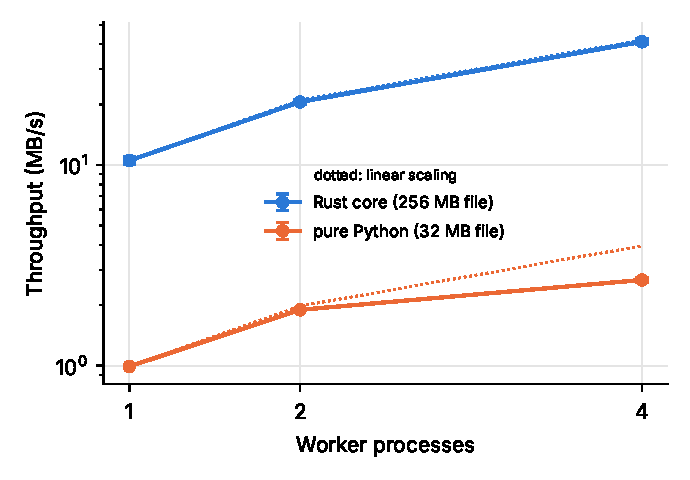
\includegraphics[width=0.62\textwidth]{fig_scaling.pdf}
\caption{Throughput of \texttt{redact\_file} against worker processes on a 4-vCPU machine, mean and standard deviation over 5 runs (log scale), on a single 256\,MB generated log file. Dotted lines show linear scaling from one worker. The parallel output is byte-identical to the sequential output (Theorem~2). The pure-Python backend on a 32\,MB file of the same kind ran at 0.99, 1.90 and 2.67\,MB/s with 1, 2 and 4 workers.}\label{f:scaling}
\end{figure}

%% ===================================================================
\section{Held-out accuracy at a glance}\label{s:accuracy}

\begin{figure}[H]
\centering
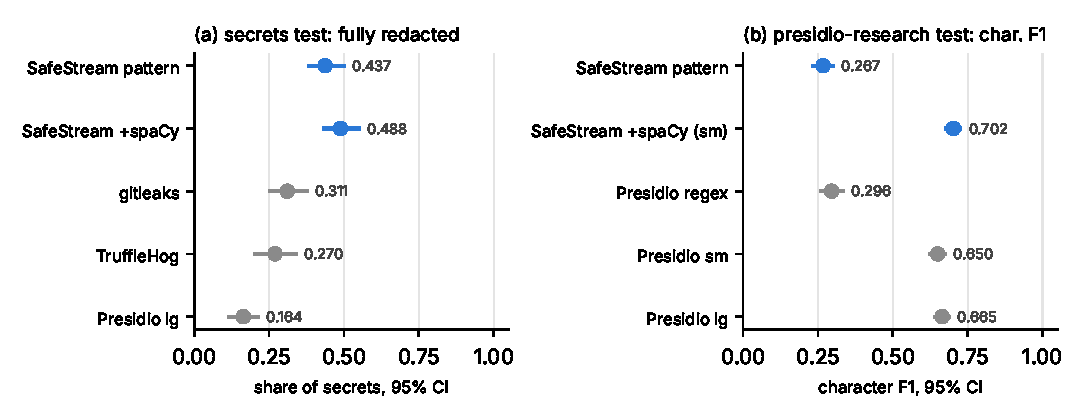
\includegraphics[width=0.9\textwidth]{fig_accuracy.pdf}
\caption{Test-split accuracy with 95\% document-level bootstrap intervals (the values of Table~4 of the article). (a) Share of secrets fully redacted on the secrets test split. (b) Character F1 on the presidio-research test split. SafeStream configurations in blue, baselines in grey.}\label{f:accuracy}
\end{figure}

%% ===================================================================
\section{Scanner sensitivity: false-positive filters disabled}\label{s:sens}

For gitleaks we removed the global allowlist and all nine per-rule allowlists, which hold its stopwords, from the release's own configuration file, leaving all 217 rules (regexes, keywords and entropy thresholds) unchanged; the unmodified file reproduced the built-in default exactly. For TruffleHog we added the results its false-positive filter drops (\texttt{--results} including \texttt{filtered\_unverified}), still without verification. Both filters-off runs are supersets of the defaults. gitleaks' filters suppressed few findings, in 6 of 313 documents, but long ones, so disabling them raised its character recall from 0.473 to 0.737 but its fully redacted rate only from 0.311 to 0.328. TruffleHog changed little. On RedactionBench, disabling the filters raised gitleaks' mandatory recall from 0.247 to 0.284 and left TruffleHog essentially unchanged; pre-exposure SafeStream exceeded both filters-off scanners in character F1 and mandatory recall under all three bootstrap schemes. The script is \texttt{benchmarks/scanner\_sensitivity.py}.

\begin{table}[ht]
\caption{Secret scanners on the secrets test split with default false-positive filters and with the filters disabled, with 95\% document-level intervals, and SafeStream's pattern tiers minus each scanner (paired, two-stage rule-clustered bootstrap). FR: fully redacted rate. \ns\ marks an interval that includes zero.}\label{t:sens}
\small
\setlength{\tabcolsep}{3pt}
\begin{tabular*}{\textwidth}{@{\extracolsep\fill}llllll}
\toprule
Scanner & Filters & Char F1 & FR & SafeStream $-$ scanner, F1 & SafeStream $-$ scanner, FR \\
\midrule
gitleaks & default & \pc{.604}{.430, .765} & \pc{.311}{.253, .375} & \pc{$+.226$}{$+.011$, $+.538$} & \pc{$+.125$}{$+.025$, $+.209$} \\
gitleaks & disabled & \pc{.805}{.664, .885} & \pc{.328}{.269, .394} & \pc{$+.039$\ns}{$-.007$, $+.141$} & \pc{$+.106$}{$+.008$, $+.193$} \\
TruffleHog & default & \pc{.306}{.204, .446} & \pc{.270}{.204, .340} & \pc{$+.530$}{$+.192$, $+.742$} & \pc{$+.184$\ns}{$-.008$, $+.363$} \\
TruffleHog & disabled & \pc{.314}{.211, .454} & \pc{.290}{.225, .363} & \pc{$+.522$}{$+.182$, $+.737$} & \pc{$+.163$\ns}{$-.028$, $+.358$} \\
\bottomrule
\end{tabular*}
\end{table}

%% ===================================================================
\section{False alarms on high-entropy non-secrets}\label{s:fp}

Before the suppression rule of Section~4.1, SafeStream flagged 83 of the 103 generated non-secrets in the development split (false-alarm rate 0.806), all through the entropy tier: every UUID, commit hash, SHA-256 digest and base64 image payload, and none of the minified JavaScript. The suppression rule was designed on the development split. A first version cost one development secret, a UUID-shaped access key assigned to \texttt{SAUCE\_ACCESS\_KEY}, which led to the secret-key veto. With the veto, the development false-alarm rate fell to 0.000 with no change in recall, and the presidio-research and RedactionBench development results were unchanged except in the fourth decimal. On the test split, the false-alarm rate fell from 0.794 [0.714, 0.872] to 0.010 [0.000, 0.035], character precision rose from 0.589 to 0.857, and recall was unchanged (0.829 character recall, 0.437 fully redacted). The test half had been scored once with the pre-fix code before the fix was made; both scores are reported. Because the gold-free documents in both halves come from the same generator, the test improvement is an optimistic estimate of the fix's effect on real non-secrets.

%% ===================================================================
\section{Where the RedactionBench leaks are}\label{s:leaks}

We re-ran five systems of Table~6 of the article (exposed pattern tiers, exposed +spaCy, gitleaks, TruffleHog and Presidio lg) on the test half at the commit that produced those rows, reproducing its mandatory recall and no-leak rates exactly, and kept the per-document predictions. The 95 test documents with mandatory gold contain 8{,}002 mandatory spans. The observations below are descriptive, from one corpus that had been inspected during development, and carry no confidence intervals.
\begin{itemize}
\item \emph{Leaks are whole misses, not boundary errors.} With spaCy, 6{,}441 mandatory spans were fully redacted, 64 partially and 1{,}497 not at all; of the 17{,}122 leaked mandatory characters, 826 (4.8\%) lie in partially redacted spans and the rest in spans with no detection. For the pattern tiers alone the share is 3.7\% (854 of 22{,}778). Presidio lg leaks more through partial coverage: 7{,}354 of its 41{,}589 leaked characters (17.7\%).
\item \emph{Few documents are near misses; leaks are concentrated.} With spaCy, 17 documents leaked nothing, 5 more leaked exactly one mandatory span and 7 more leaked two, so fixing one or two spans per document would raise the no-leak rate to at most 29 of 95 (0.305). The median document leaked 6 mandatory spans (interquartile range 2--16), a median of 23\% of its mandatory spans, and the 9 documents with the most leaked characters held 67\% of them. For the pattern tiers alone the median document leaked 11 spans (52\%), and only 2 documents were within two spans of no leak.
\item \emph{What is missed.} The corpus carries no entity types, so we grouped spans by a coarse shape heuristic. Capitalised words (largely names) leaked at a rate of 0.90 without a named-entity model and 0.27 with spaCy, which accounts for most of the gap between the two configurations. Spans containing \texttt{@} leaked at 0.95 (36 of 38) with spaCy; inspection of a few of them, after all scores were final, showed passwords inside connection strings or quoted configuration values that the e-mail pattern split or that no tier matched. No code was changed in response.
\item \emph{Union of systems.} An oracle that took the union of all five systems' redactions would still leave 69 of 95 documents leaking (no-leak rate 0.274).
\end{itemize}
As an illustration only, if a document had $n$ independent must-redact units each detected with probability $p$, it would be leak-free with probability $p^{n}$, which for $n$ in the hundreds is small even for $p$ close to one. Real misses are correlated, so this is not a model of the data, but it shows why per-character recall in the 0.68--0.76 range is compatible with almost no fully protected documents.

%% ===================================================================
\section{Ablation}\label{s:ablation}

\begin{table}[ht]
\caption{Ablation on the test splits (pure-Python backend, identical output to the Rust core). Paired differences against the full pattern pipeline, with 95\% document-level intervals.}\label{t:ablation}
\small
\begin{tabular*}{\textwidth}{@{\extracolsep\fill}llll}
\toprule
Change & secrets & presidio-research & RedactionBench \\
\midrule
\multicolumn{4}{@{}l}{\emph{Character F1, full pattern pipeline minus variant}}\\
Remove entropy tier & $+.455$ [$.242$, $.641$] & $.000$ & $+.156$ [$.104$, $.224$] \\
Remove label-anchored tier & $.000$ & $+.030$ [$.019$, $.044$] & $+.004$ [$.002$, $.006$] \\
Remove contextual detections & $.000$ & $.000$ & $.000$ \\
\midrule
\multicolumn{4}{@{}l}{\emph{Union rule versus greedy resolution (with spaCy), union minus greedy}}\\
Character recall & $+.006$ [$.000$, $.017$] & $+.005$ [$.002$, $.008$] & $+.009$ [$.004$, $.016$] \\
FR or mandatory recall$^{a}$ & $+.013$ [$.000$, $.032$] & $+.001$ [$.000$, $.002$] & $+.012$ [$.004$, $.022$] \\
\bottomrule
\end{tabular*}

\smallskip
\footnotesize $^{a}$Fully redacted rate (FR) for secrets and presidio-research; mandatory recall for RedactionBench.
\end{table}

The entropy tier carried most of the credential recall: without it, character F1 on secrets fell from 0.842 to 0.383. The label-anchored tier mattered on presidio-research, where several identifiers carry labels. The contextual scorer's own detections changed no result on these corpora; its confidence adjustment was kept in every variant. Alone, the deterministic tier reached a character F1 of 0.380 on secrets and 0.237 on presidio-research, and the entropy tier alone 0.822 on secrets. The union rule raised recall by small and mostly significant amounts at no significant cost in F1 on secrets ($+0.000$ [$-0.003$, $+0.005$]) and RedactionBench ($+0.003$ [$-0.002$, $+0.008$]); on presidio-research its F1 difference was $+0.004$ [$+0.001$, $+0.007$]. The ablation was not planned and its intervals are document-level only.

%% ===================================================================
\section{TAB: character recall by entity type}\label{s:tab}

Table~\ref{t:tab} breaks down the character recall of Table~10 of the article by TAB's entity types, pooled over document--annotator pairs (descriptive; no intervals). The secret scanners redacted nothing and are omitted. SafeStream's named-entity tier maps only spaCy's person, organisation and place labels, so it leaves dates, which are 44.7\% of the gold characters, almost entirely unredacted; its opt-in date tier, evaluated separately, redacts most of them.

\begin{table}[ht]
\caption{Character recall on TAB by entity type (\textsc{direct} and \textsc{quasi} mentions). Share: the type's share of gold characters.}\label{t:tab}
\small
\setlength{\tabcolsep}{4pt}
\begin{tabular*}{\textwidth}{@{\extracolsep\fill}lrrrrrrr}
\toprule
Type & Share (\%) & Pattern & +dates & +spaCy & P.\ regex & P.\ sm & P.\ lg \\
\midrule
\textsc{datetime} & 44.7 & 0.01 & 0.88 & 0.01 & 0.00 & 0.98 & 0.99 \\
\textsc{person} & 19.8 & 0.00 & 0.00 & 0.78 & 0.06 & 0.72 & 0.79 \\
\textsc{org} & 13.9 & 0.00 & 0.00 & 0.78 & 0.07 & 0.21 & 0.22 \\
\textsc{loc} & 5.2 & 0.03 & 0.03 & 0.87 & 0.07 & 0.78 & 0.76 \\
\textsc{code} & 4.7 & 0.00 & 0.00 & 0.03 & 0.01 & 0.12 & 0.07 \\
\textsc{misc} & 4.5 & 0.00 & 0.01 & 0.10 & 0.08 & 0.14 & 0.15 \\
\textsc{dem} & 4.0 & 0.00 & 0.00 & 0.15 & 0.07 & 0.44 & 0.47 \\
\textsc{quantity} & 3.2 & 0.00 & 0.00 & 0.12 & 0.03 & 0.05 & 0.04 \\
\bottomrule
\end{tabular*}
\end{table}

%% ===================================================================
\section{TAB held-out judgments: character recall by entity type}\label{s:tabtrain}

Table~\ref{t:tabtrain} breaks down the held-out results of Table~11 of the article (TAB training split, 1,014 judgments) by entity type, pooled over document--annotator pairs (descriptive; no intervals). The free-text configuration is \texttt{Redactor(profile="prose", use\_ner=True)} frozen at commit \texttt{9c10975}; its protocol is \texttt{benchmarks/TAB\_PROSE\_PROTOCOL.md}.

\begin{table}[ht]
\caption{Character recall on held-out TAB judgments by entity type (\textsc{direct} and \textsc{quasi} mentions).}\label{t:tabtrain}
\small
\begin{tabular*}{\textwidth}{@{\extracolsep\fill}lrrrrr}
\toprule
Type & Free-text & +spaCy & P.\ regex & P.\ sm & P.\ lg \\
\midrule
\textsc{datetime} & 0.94 & 0.00 & 0.00 & 0.98 & 0.98 \\
\textsc{person} & 0.88 & 0.77 & 0.03 & 0.71 & 0.79 \\
\textsc{org} & 0.84 & 0.83 & 0.09 & 0.16 & 0.17 \\
\textsc{loc} & 0.82 & 0.81 & 0.09 & 0.69 & 0.72 \\
\textsc{code} & 0.91 & 0.02 & 0.02 & 0.07 & 0.04 \\
\textsc{misc} & 0.17 & 0.15 & 0.07 & 0.16 & 0.16 \\
\textsc{dem} & 0.26 & 0.07 & 0.10 & 0.36 & 0.37 \\
\textsc{quantity} & 0.49 & 0.10 & 0.03 & 0.08 & 0.05 \\
\bottomrule
\end{tabular*}
\end{table}

%% ===================================================================
\section{CredData: fully redacted rate by credential category}\label{s:cred}

Table~\ref{t:cred} breaks down the fully redacted rate of Table~5 of the article by CredData's first category label (descriptive; no intervals; the 14 most frequent categories, which hold 13,566 of the 14,626 values). Evaluated: SafeStream's pattern tiers at commit \texttt{3d2c6ac}; current: the default profile at \texttt{9c10975}. The protocol is \texttt{benchmarks/CREDDATA\_PROTOCOL.md}.

\begin{table}[ht]
\caption{Fully redacted rate on CredData by category.}\label{t:cred}
\small
\begin{tabular*}{\textwidth}{@{\extracolsep\fill}lrrrrr}
\toprule
Category & Values & Evaluated & Current & gitleaks & TruffleHog \\
\midrule
Key & 4,015 & 0.94 & 0.96 & 0.86 & 0.00 \\
Password & 2,655 & 0.19 & 0.88 & 0.05 & 0.00 \\
UUID & 2,356 & 0.09 & 0.11 & 0.01 & 0.00 \\
Secret & 1,343 & 0.77 & 0.89 & 0.81 & 0.00 \\
Auth & 1,095 & 0.73 & 0.78 & 0.11 & 0.00 \\
Token & 798 & 0.47 & 0.78 & 0.60 & 0.00 \\
API & 226 & 0.33 & 0.49 & 0.24 & 0.00 \\
URL credentials & 213 & 0.96 & 0.96 & 0.00 & 0.29 \\
AWS client ID & 198 & 0.75 & 0.75 & 0.46 & 0.02 \\
JSON Web Token & 152 & 0.97 & 0.99 & 0.92 & 0.00 \\
PEM private key & 151 & 0.90 & 0.91 & 1.00 & 0.00 \\
Nonce & 149 & 0.68 & 0.68 & 0.00 & 0.00 \\
NTLM token & 117 & 1.00 & 1.00 & 0.00 & 0.00 \\
Credential & 94 & 0.10 & 0.14 & 0.07 & 0.03 \\
\bottomrule
\end{tabular*}
\end{table}

%% ===================================================================
\section{Implementation mapping of the proofs}\label{s:mapping}

Table~\ref{t:mapping} maps each step of the proofs of Theorems~1--3 (Section~5 and Appendix~A of the article) to the code that discharges it.

\begin{table}[ht]
\caption{Proof steps and the code that discharges them. Module paths are relative to \texttt{src/\allowbreak safestream\_\allowbreak redactor/}.}\label{t:mapping}
\small
\begin{tabular*}{\textwidth}{@{\extracolsep\fill}>{\raggedright\arraybackslash}p{0.40\textwidth}>{\raggedright\arraybackslash}p{0.54\textwidth}}
\toprule
Proof step & Code and tests \\
\midrule
Declared $(L_d, C_{\mathrm{left},d}, C_{\mathrm{right},d})$ and $\max(L_d + C_{\mathrm{right},d}, C_{\mathrm{left},d})$ & \texttt{detectors/base.py}: \texttt{StreamingRequirements}, \texttt{required\_overlap} \\
$w^{\star}$ (Eq.~1); refusal below it & \texttt{engine.required\_overlap}; \texttt{Redactor.min\_safe\_overlap} \\
Window $P \cdot B$, spans inside $P$ dropped & \texttt{engine.stream\_windows}, \texttt{window\_detect} \\
Planned boundary and retreat & \texttt{emit\_upto = len(buffer) - overlap}; \texttt{\_retreat\_boundary} \\
Span longer than $w$ fails closed & \texttt{\_check\_overlong} (\texttt{strict\_spans}) \\
Coalescing to $m$; pinned branch & \texttt{min\_emit}, \texttt{need} in \texttt{stream\_windows} \\
Disjoint detection set & \texttt{entities.resolve\_overlaps} \\
Span-local rewrite & \texttt{policy.RedactionPolicy.apply}, \texttt{render} \\
Ranges of at least $4w$ & \texttt{parallel.plan\_ranges} \\
Context and padding of $X_r$ & \texttt{parallel.\_redact\_range}, \texttt{\_read\_chars\_before}, \texttt{\_read\_chars\_after} \\
Straddler reports; cuts $\ell_r$, $u_r$ & \texttt{parallel.\_find\_straddler}; \texttt{start\_cut}, \texttt{end\_cut} \\
Holdback of $2w$ & \texttt{flush(cursor - 2 * ov)} in \texttt{\_redact\_range} \\
Seam valve and fallback & \texttt{redact\_file\_parallel}: \texttt{left.end\_seam != right.start\_seam} \\
Empirical corroboration & \texttt{tests/test\_streaming.py}, \texttt{test\_properties.py}, \texttt{test\_parallel.py}, \texttt{test\_streaming\_contract.py}, \texttt{test\_formal\_constants.py}, \texttt{test\_memory.py} \\
\bottomrule
\end{tabular*}
\end{table}

\end{document}
